\documentclass[12pt,a4paper,oneside]{report}

% ============================================================
% RBU B.TECH PROJECT REPORT - SAMPLE LATEX TEMPLATE
% Based on the official Project Report Format and Submission
% Guidelines provided by the School of Computer Science and
% Engineering, Ramdeobaba University.
%
% Compile with XeLaTeX or LuaLaTeX.
% ============================================================

\usepackage[a4paper,left=1.5in,right=1in,top=1in,bottom=1in]{geometry}
\usepackage{fontspec}
\IfFontExistsTF{Times New Roman}
  {\setmainfont{Times New Roman}}
  {\setmainfont{Liberation Serif}}
\usepackage{setspace}
\onehalfspacing

\usepackage{graphicx}
\usepackage{booktabs}
\usepackage{array}
\usepackage{longtable}
\usepackage{amsmath,amssymb}
\usepackage{caption}
\usepackage{float}
\usepackage{enumitem}
\usepackage{url}
\usepackage[hidelinks]{hyperref}
\usepackage{fancyhdr}
\usepackage{titlesec}
\usepackage{tocloft}
\usepackage{chngcntr}
\usepackage{ragged2e}
\usepackage{multirow}
\usepackage{tikz}
\usepackage{lipsum}

% ------------------------------------------------------------
% Paragraph formatting
% ------------------------------------------------------------
\setlength{\parindent}{0pt}
\setlength{\parskip}{6pt}
\justifying

% ------------------------------------------------------------
% Chapter / Section formatting
% ------------------------------------------------------------
\titleformat{\chapter}
  {\normalfont\bfseries\fontsize{16}{19}\selectfont}
  {\thechapter.}{0.5em}{\MakeUppercase}

\titleformat{\section}
  {\normalfont\bfseries\fontsize{14}{17}\selectfont}
  {\thesection}{0.7em}{}

\titleformat{\subsection}
  {\normalfont\bfseries\fontsize{12}{15}\selectfont}
  {\thesubsection}{0.7em}{}

\titleformat{\subsubsection}
  {\normalfont\bfseries\fontsize{12}{15}\selectfont}
  {\thesubsubsection}{0.7em}{}

% ------------------------------------------------------------
% Chapter-wise figures, tables and equations
% ------------------------------------------------------------
\counterwithin{figure}{chapter}
\counterwithin{table}{chapter}
\counterwithin{equation}{chapter}

\captionsetup[figure]{
    font={rm,small},
    labelfont=bf,
    justification=centering,
    position=bottom
}
\captionsetup[table]{
    font={rm,small},
    labelfont=bf,
    justification=centering,
    position=top
}

% ------------------------------------------------------------
% Header / Footer
% ------------------------------------------------------------
\pagestyle{fancy}
\fancyhf{}
\renewcommand{\headrulewidth}{0pt}
\fancyfoot[C]{\thepage}

% No page number on the first page of each chapter
\fancypagestyle{plain}{
    \fancyhf{}
    \renewcommand{\headrulewidth}{0pt}
    \fancyfoot[C]{\thepage}
}

% ------------------------------------------------------------
% Chapter separator
% ------------------------------------------------------------
\newcommand{\chapterseparator}{
    \clearpage
    \thispagestyle{empty}
    \begin{center}
        \vspace*{5cm}
        \rule{0.65\textwidth}{0.5pt}\\[1.2cm]
        {\fontsize{16}{20}\selectfont\bfseries CHAPTER}\\[0.8cm]
        {\fontsize{24}{28}\selectfont\bfseries \the\numexpr\value{chapter}+1\relax}\\[1.2cm]
        \rule{0.65\textwidth}{0.5pt}
    \end{center}
    \clearpage
}

% ------------------------------------------------------------
% Sample figure placeholder
% ------------------------------------------------------------
\newcommand{\samplefigure}[2][0.75\textwidth]{
\begin{figure}[H]
    \centering
    \fbox{
        \begin{minipage}[c][5cm][c]{#1}
            \centering
            \textit{Insert project figure / architecture diagram here}\\[6pt]
            \small #2
        \end{minipage}
    }
    \caption{#2}
\end{figure}
}

% ------------------------------------------------------------
% Document
% ------------------------------------------------------------
\begin{document}

% ============================================================
% COVER PAGE
% ============================================================
\begin{titlepage}
\thispagestyle{empty}
\begin{center}

{\fontsize{16}{19}\selectfont\bfseries RAMDEOBABA UNIVERSITY}\\[0.35cm]

{\fontsize{14}{17}\selectfont\bfseries SCHOOL OF COMPUTER SCIENCE AND ENGINEERING}\\[0.8cm]


\includegraphics[height=3.2cm]{figures/rbu_logo.png}\\[0.8cm]

{\fontsize{14}{17}\selectfont\bfseries
B. TECH PROJECT REPORT\\
(Major/Honor/Minor/Idea Lab/External)}\\[0.5cm]

ON\\[0.5cm]

{\fontsize{17}{21}\selectfont\bfseries
I-JEPA-AD: DECODER-FREE LATENT ANOMALY DETECTION WITH COARSE-TO-FINE ADAPTIVE MASKING}\\[1.0cm]

{\fontsize{13}{16}\selectfont Submitted by}\\[0.5cm]

\begin{tabular}{ll}
Aryan Jawanjal & (Roll No. A-35)\\
Akshat Tiwari & (Roll No. A-11)\\
Arnav Milmile & (Roll No. A-30)\\
Aashutosh Dubey & (Roll No. A-02)
\end{tabular}\\[1.0cm]

{\fontsize{13}{16}\selectfont Under the Guidance of}\\[0.4cm]
{\fontsize{13}{16}\selectfont\bfseries Dr. Sunita G. Rawat}\\[0.9cm]

{\fontsize{12}{15}\selectfont Academic Year: 2026--2027}

\vfill

{\fontsize{11}{14}\selectfont
School of Computer Science and Engineering\\
Ramdeobaba University, Nagpur}

\end{center}
\end{titlepage}

% ============================================================
% FRONT MATTER
% ============================================================
\pagenumbering{roman}

% Student Declaration
\chapter*{STUDENT DECLARATION}
\addcontentsline{toc}{chapter}{Student Declaration}

We hereby declare that the project report entitled
\textbf{``I-JEPA-AD: Decoder-Free Latent Anomaly Detection with Coarse-to-Fine Adaptive Masking''}
is submitted as part of the requirements for the B.Tech programme at
Ramdeobaba University.

The work presented in this report is our own work carried out under the
guidance of the project supervisor. All external sources, datasets,
software tools, figures and technical material used in the project have
been appropriately acknowledged and cited.

\vspace{1cm}

\begin{flushright}
Aryan Jawanjal\\
Roll No. A-35\\[0.5cm]
Akshat Tiwari\\
Roll No. A-11\\[0.5cm]
Arnav Milmile\\
Roll No. A-30\\[0.5cm]
Aashutosh Dubey\\
Roll No. A-02
\end{flushright}

% Approval Sheet
\chapter*{APPROVAL SHEET}
\addcontentsline{toc}{chapter}{Approval Sheet}

This is to certify that the project report entitled
\textbf{``I-JEPA-AD: Decoder-Free Latent Anomaly Detection with Coarse-to-Fine Adaptive Masking''}
has been carried out by the students listed below under the guidance of
the undersigned and is submitted in partial fulfilment of the academic
requirements of the B.Tech programme.

\vspace{0.5cm}

Aryan Jawanjal, Akshat Tiwari, Arnav Milmile, Aashutosh Dubey

\vspace{1.2cm}

\begin{center}
\begin{tabular}{ccc}
\shortstack{Guide\\Dr. Sunita G. Rawat} & \shortstack{Project In-Charge\\\phantom{x}} & \shortstack{Associate Head\\\phantom{x}}\\[1.2cm]
(Signature) & (Signature) & (Signature)
\end{tabular}

\vspace{1.2cm}

\begin{tabular}{cc}
Dean, CSE & External Examiner\\[1.2cm]
(Signature) & (Signature)
\end{tabular}
\end{center}

% Acknowledgement
\chapter*{ACKNOWLEDGEMENT}
\addcontentsline{toc}{chapter}{Acknowledgement}

We express our sincere gratitude to Ramdeobaba University and the
School of Computer Science and Engineering for providing the academic
environment and facilities required to complete this project.

We are grateful to our project guide, Dr. Sunita G. Rawat, for continuous
guidance, technical suggestions and constructive feedback throughout the
project. We also thank the Project In-Charge, Associate Head and Dean,
School of Computer Science and Engineering, for their support.

We acknowledge the authors of I-JEPA and of the MVTec AD dataset, whose
public models and data made this study possible. Finally, we thank our
classmates, friends and family members who contributed directly or
indirectly to the successful completion of this work.

% Abstract
\chapter*{ABSTRACT}
\addcontentsline{toc}{chapter}{Abstract}

Unsupervised visual anomaly detection for industrial inspection is
dominated by pixel-reconstruction models, which need heavy decoders, and
by nearest-neighbour feature banks, whose memory grows with the training
set. This project studies a third option, I-JEPA-AD: a decoder-free
detector that predicts masked image regions entirely in the latent space
of a frozen I-JEPA ViT-g/16 encoder. A small Transformer predictor is
trained only on cached latents of defect-free images, and anomalies are
scored by the cosine discrepancy between predicted and actual latents. A
coarse-to-fine masking scheme evaluates sixteen coarse blocks first and
runs single-patch fine masks only where a gate flags a suspicious region.

On a three-category pilot of MVTec AD (bottle, capsule, hazelnut) the
original pipeline reaches a mean pixel AUROC of 0.840 with about 16 masks
per image, a 92 percent reduction from 196 dense masks, and an end-to-end
latency of 134 ms against 350 ms for dense masking on an 8 GB RTX 4060.
However, the fine stage almost never fires with the default gate, capsule
stays near chance, and a nearest-neighbour baseline on the same latents is
stronger. We then choose settings on synthetic defects pasted onto nominal
validation images, never on the test split. Using mid-level encoder tokens
(layer 32 of 40) and normalising scores per token position raises the mean
top-3 image AUROC from 0.787 to 0.920, the mean pixel AUROC from 0.840 to
0.962 and the mean AUPRO from 0.480 to 0.813 at the same 16 masks per
image, with paired-bootstrap improvements over the original pipeline in all
three categories. The report also documents negative results and the
limitations of the pilot.

\textbf{Keywords:} Anomaly Detection, I-JEPA, Latent Prediction, Masked
Modelling, Industrial Inspection, MVTec AD

% Table of Contents
\tableofcontents
\clearpage

\listoffigures
\clearpage

\listoftables
\clearpage

% Abbreviations
\chapter*{LIST OF ABBREVIATIONS}
\addcontentsline{toc}{chapter}{List of Abbreviations}

\begin{tabular}{ll}
AUROC & Area Under the Receiver Operating Characteristic curve\\
AUPRO & Area Under the Per-Region-Overlap curve\\
GPU & Graphics Processing Unit\\
I-JEPA & Image-based Joint-Embedding Predictive Architecture\\
kNN & k-Nearest Neighbour (here, nearest-neighbour feature bank)\\
MAE & Masked Autoencoder\\
MVTec AD & MVTec Anomaly Detection dataset\\
RBU & Ramdeobaba University\\
SHA & Secure Hash Algorithm\\
UI & User Interface\\
ViT & Vision Transformer
\end{tabular}

% ============================================================
% MAIN MATTER
% ============================================================
\clearpage
\pagenumbering{arabic}

% ------------------------------------------------------------
% CHAPTER 1
% ------------------------------------------------------------
\chapterseparator
\chapter{Introduction}

\section{Background}

Automated detection and localisation of surface defects is central to
industrial quality control. Defective samples are rare, and the types of
defect that may appear are open-ended, so the standard setting is
\emph{unsupervised}: a model is trained on defect-free (nominal) images
only and must flag anything that deviates from them at test time
\cite{bergmann2019mvtec,bergmann2021mvtec}. The MVTec AD dataset is the
usual benchmark for this task.

Two families of methods dominate. Reconstruction-based approaches
(autoencoders, generative networks, masked autoencoders and inpainting
networks) assume that anomalies cannot be reconstructed well
\cite{he2022mae,zavrtanik2021inpainting,zavrtanik2021draem}. They pay for a
pixel decoder, spend capacity on irrelevant high-frequency texture, and can
generalise so well that they reconstruct the defect. Embedding-based
approaches such as PaDiM and PatchCore compare test patch features with
those of nominal images \cite{defard2021padim,roth2022patchcore}. They are
accurate, but PatchCore stores a memory bank whose size scales with the
number of training patches.

The Joint-Embedding Predictive Architecture (I-JEPA) offers a different
route: a model learns to predict the \emph{representations} of masked image
blocks from visible context, without ever generating pixels
\cite{assran2023ijepa,lecun2022path}. This suggests an anomaly detector with
no decoder, in which a region is anomalous when its latent representation
cannot be predicted from its surroundings.

\section{Problem Statement}

Given only defect-free images of an object category, the task is to decide
whether a new image contains a defect (image-level detection) and to
indicate where it is (pixel-level localisation). Using I-JEPA for this
raises two practical issues. First, evaluating the predictor over every
patch with a dense sliding window is redundant, since most of an industrial
image is nominal. Second, the frozen ViT-g/16 backbone has about one billion
parameters, so training and inference must fit a consumer GPU with 8~GB of
memory.

\section{Objectives}

The objectives of the project are:
\begin{itemize}[leftmargin=*]
    \item To build a decoder-free pipeline that caches frozen I-JEPA
    ViT-g/16 latents offline, trains a lightweight Transformer predictor on
    nominal latents only, and scores anomalies by cosine discrepancy.
    \item To design a coarse-to-fine inference scheme that spends predictor
    passes only where a gate flags a suspicious region.
    \item To define a validation-only protocol for choosing settings, so
    that no choice is tuned on the test labels.
    \item To measure accuracy, number of predictor passes, latency and GPU
    memory against fixed-mask, dense-mask and nearest-neighbour references.
    \item To improve the detector through choices made on synthetic
    validation data, and to report negative results honestly.
\end{itemize}

\section{Scope of the Project}

The study is a pilot on three of the fifteen MVTec AD categories (bottle,
capsule and hazelnut) at the native $224\times224$ input size, with a frozen
encoder and a single consumer GPU. The remaining twelve categories, MVTec AD
2, a faithful PatchCore and MAE baseline, multi-seed runs and higher input
resolution are outside the scope of the work reported here and are listed as
future scope. The results are therefore pilot evidence and not a benchmark
claim.

\section{Organization of the Report}

Chapter~2 reviews related work and states the research gap. Chapter~3
describes the proposed system and the methodology, including the
validation-based selection protocol. Chapter~4 covers the system design and
implementation. Chapter~5 presents the experimental setup, results,
discussion and limitations. Chapter~6 concludes and lists future scope.
Appendices give the publication status, the contribution of each student and
the project outputs.

\chapterseparator
\chapter{Literature Review and Research Gap}

\section{Introduction}

This chapter reviews the families of unsupervised anomaly detection
methods that are relevant to the project and identifies the gap that
motivates a latent-prediction detector.

\section{Existing Approaches}

\textbf{Reconstruction-based detection.} Autoencoder, generative and
masked-autoencoder (MAE) detectors reconstruct nominal images and score by
reconstruction error \cite{he2022mae,zavrtanik2021draem}. Reconstruction by
inpainting reduces the tendency to reconstruct defects by hiding regions
before reconstruction \cite{zavrtanik2021inpainting}. All of these need a
decoder that operates in pixel space.

\textbf{Embedding-based detection.} PaDiM models per-position Gaussian
statistics of pretrained features \cite{defard2021padim}. PatchCore stores a
coreset of nominal patch features and scores a test patch by its
nearest-neighbour distance \cite{roth2022patchcore}. EfficientAD targets
millisecond-level latency with a lightweight student--teacher design
\cite{batzner2024efficientad}. Libraries such as Anomalib standardise the
evaluation of these methods \cite{akcay2022anomalib}.

\textbf{Joint-embedding prediction.} I-JEPA learns by predicting
target-block representations from a context block in latent space, which
avoids pixel-level detail and hand-crafted augmentations
\cite{assran2023ijepa}. Its use for \emph{anomaly localisation}, and in
particular how to spend predictor evaluations economically, has received
little study.

\textbf{Synthetic defects.} Pasting or blending synthetic defects onto
normal images is an established way to obtain labelled anomalies without
real defect data; CutPaste and DRAEM are well-known examples
\cite{li2021cutpaste,zavrtanik2021draem}. In this project such defects are
used only to choose settings, never to train the detector.

\section{Comparison of Existing Approaches}

\begin{table}[H]
\centering
\caption{Comparison of unsupervised anomaly detection approaches.}
\begin{tabular}{p{0.20\textwidth}p{0.20\textwidth}p{0.15\textwidth}p{0.28\textwidth}}
\toprule
Approach & Principle & Needs pixel decoder & Main limitation\\
\midrule
Reconstruction (AE, MAE, inpainting) & Reconstruct input; score the error & Yes & Defects may be reconstructed; capacity spent on texture\\
PaDiM & Per-position Gaussian of pretrained features & No & Fixed statistics may be too coarse for small defects\\
PatchCore & Nearest neighbour to a bank of nominal patches & No & Memory grows with training patches\\
I-JEPA-AD (this work) & Predict masked latents; score the discrepancy & No & Many predictor passes; weaker than a bank in this pilot\\
\bottomrule
\end{tabular}
\end{table}

\section{Limitations of Existing Work}

Decoder-based methods carry the cost and the failure modes of pixel
reconstruction. Feature-bank methods are strong but trade memory for
accuracy, and their memory footprint grows with the amount of nominal data.
Methods based on latent prediction have not been studied systematically for
localisation, and there is no established way to decide where the
(expensive) predictor should be evaluated.

\section{Research Gap}

To the authors' knowledge, a frozen I-JEPA predictor has not been studied as a
decoder-free anomaly detector with an adaptive masking policy and a protocol
that selects its settings without touching the test labels. This project
addresses that gap with a measured comparison of masking policies, a
validation-only selection protocol and an explicit account of where the
approach fails.

% ------------------------------------------------------------
% CHAPTER 3
% ------------------------------------------------------------
\chapterseparator
\chapter{Proposed System and Methodology}

\section{Proposed System}

Figure~\ref{fig:arch} gives an overview. The I-JEPA encoder is frozen
throughout and only the predictor is trained. Latents of nominal images are
computed once and cached; the predictor is trained on the cache. At test
time a coarse pass is followed by a gated fine pass and the two score maps
are fused into a heat map and an image score.

\begin{figure}[H]
\centering
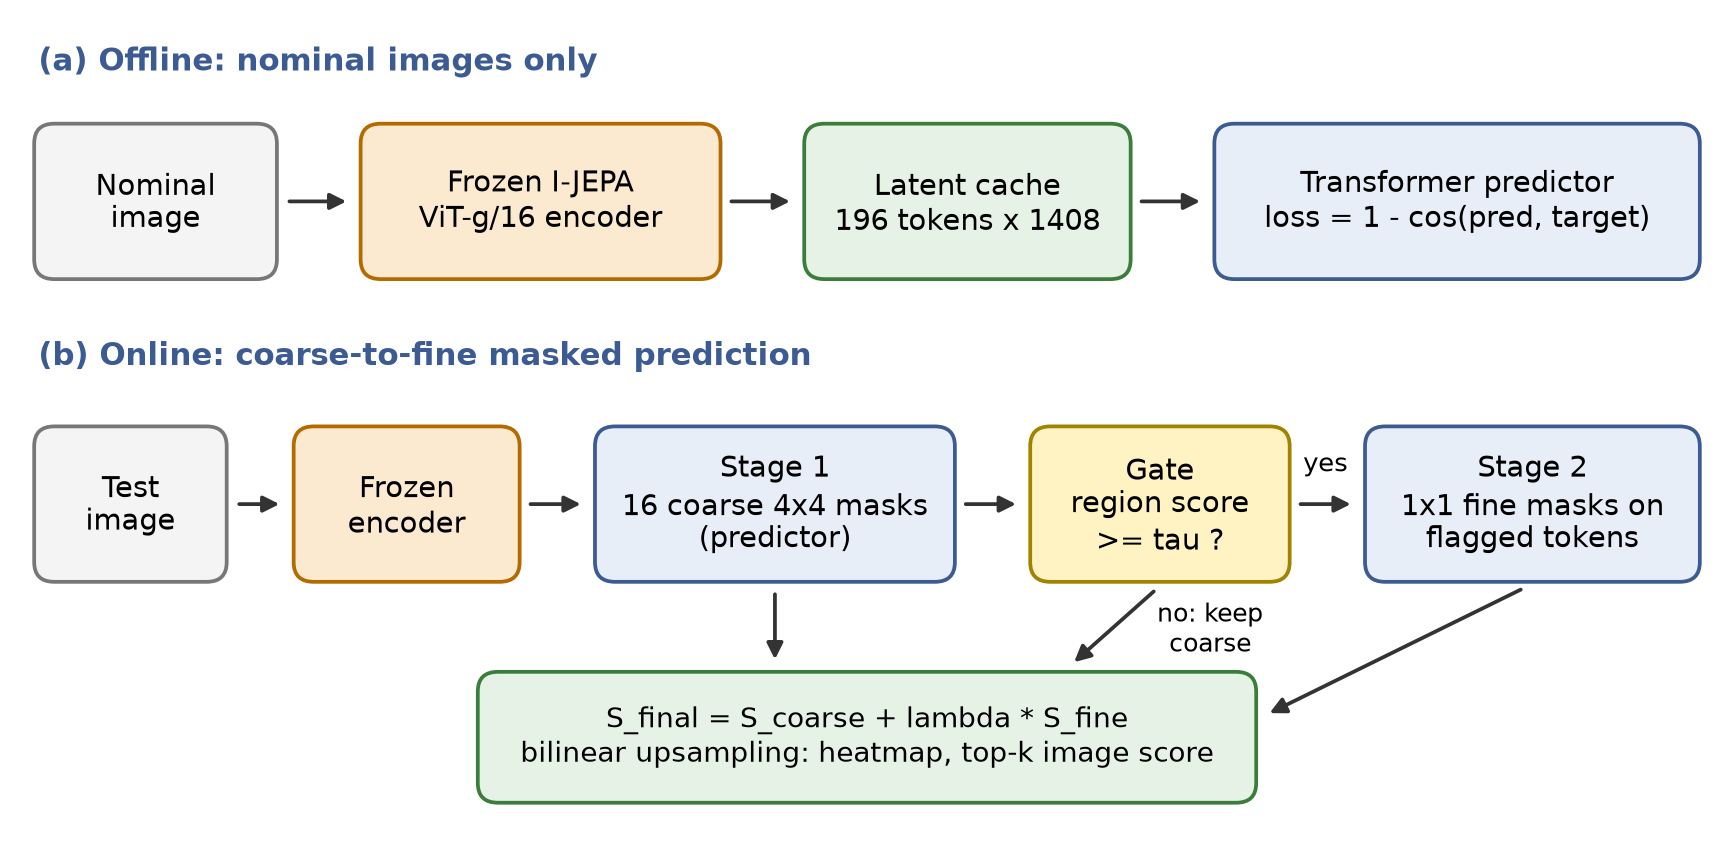
\includegraphics[width=0.95\textwidth]{figures/architecture.png}
\caption{I-JEPA-AD overview. (a) Latents of nominal images are cached once
and used to train the predictor. (b) At test time a coarse pass is followed
by a gated fine pass, and the two score maps are fused.}
\label{fig:arch}
\end{figure}

\section{Data Acquisition}

The pilot uses the categories \emph{bottle}, \emph{capsule} and
\emph{hazelnut} of MVTec AD \cite{bergmann2019mvtec}. The official training
set (nominal images only) is split by image-content hash into 90\,\%
predictor-training images and 10\,\% validation images (seed 0). The
validation images are used only for early stopping, calibration and
selection; the official test set is touched only for final metrics.
Table~\ref{tab:data} lists the sizes. The split was verified to have no
overlap between training, validation and test images.

\begin{table}[H]
\centering
\caption{Pilot split sizes (images).}
\label{tab:data}
\resizebox{\textwidth}{!}{%
\begin{tabular}{lrrrrr}
\hline
\textbf{Category} & \textbf{Train} & \textbf{Val} & \textbf{Test} & \textbf{Test good} & \textbf{Test defect} \\
\hline
Bottle   & 188 & 21 & 83  & 20 & 63 \\
Capsule  & 197 & 22 & 132 & 23 & 109 \\
Hazelnut & 352 & 39 & 110 & 40 & 70 \\
\hline
\end{tabular}%
}

\end{table}

\section{Data Preprocessing and Latent Cache}

An image is resized to $224\times224$ and normalised with ImageNet
statistics. The official I-JEPA ViT-g/16 (ImageNet-22K) target encoder, with
about $1.01\times10^{9}$ parameters, maps it to a $14\times14$ grid of 196
patch tokens $z_i\in\mathbb{R}^{1408}$. Since the encoder is frozen, every
image is encoded once and the latents are stored in a cache whose identity
includes the checkpoint hash, the preprocessing specification and the
SHA-256 of the image content. This decouples predictor training from the
16.5~GB checkpoint and keeps training within an 8~GB budget.

\section{Analytical Method}

\subsection{Latent predictor}

The predictor receives all 196 latents together with a binary target mask
$m\in\{0,1\}^{196}$. Masked tokens are replaced by a learned mask token, a
learned positional embedding is added, and a Transformer encoder (hidden
size 512, 4 layers, 8 heads, about 14\,M parameters) outputs a prediction
$\hat z_i\in\mathbb{R}^{1408}$ for every token. The model is trained on
nominal images only with the cosine loss
\begin{equation}
\mathcal{L}=\frac{1}{|M|}\sum_{i\in M}\bigl(1-\cos(\hat z_i, z_i)\bigr),
\end{equation}
where $M$ is the set of masked tokens and the target $z_i$ is the cached
latent. The loss is evaluated on masked tokens only, and the masked input is
replaced by the mask token before any computation, so target latents cannot
reach the predictor.

\textbf{Inference-aligned training masks.} Inference scores either one
$4\times4$ coarse block or single tokens, so training masks follow the same
geometry: with probability 0.5 a row hides one of the grid-aligned
$4\times4$ windows, otherwise it hides up to eight mutually non-adjacent
single tokens.

\subsection{Coarse-to-fine inference}

The anomaly score of a token is the cosine discrepancy
$s_i = 1-\cos(\hat z_i, z_i)\in[0,2]$.

\textbf{Stage 1 (coarse).} The grid is partitioned into 16 non-overlapping
$4\times4$ windows. Each window is masked in turn and the predictor yields
$s_i$ for its tokens, giving the coarse map $S_{\mathrm{coarse}}$ with 16
predictor passes. The region score $r_i$ of a token is the mean coarse score
of its window.

\textbf{Stage 2 (adaptive fine).} Every token whose region score satisfies
$r_i\ge\tau$ receives its own $1\times1$ mask and an extra predictor pass,
giving $S_{\mathrm{fine}}$ (zero elsewhere). If the gate never fires, the
method reduces to fixed coarse masking; if it fires everywhere, it becomes
dense masking with 196 single-token masks.

\textbf{Fusion and image score.} The final map is
\begin{equation}
S_{\mathrm{final}}=S_{\mathrm{coarse}}+\lambda\,S_{\mathrm{fine}},
\end{equation}
bilinearly upsampled to image resolution for pixel-level evaluation. The
image score is the maximum of $S_{\mathrm{final}}$ or the mean of its $k$
largest values (top-$k$).

\textbf{Cost model.} Fixed masking costs 16 predictor passes, dense masking
196 and adaptive masking $16+n_f$, where $n_f$ is the number of tokens
passing the gate. The encoder runs once per image in all cases.

\section{Validation-Based Selection Protocol}

The nominal validation images contain no defects, so nothing can be chosen
for \emph{detection} quality from them alone. The project therefore builds a
labelled synthetic validation set and uses it, with a fixed protocol, to
choose settings without reading the test split.

\textbf{Synthetic-defect set.} For every nominal validation image four
defects are generated with a fixed seed, alternating CutPaste scars and
DRAEM-style Perlin-noise texture blends. Defects stay on the object and
cover 0.3--4\,\% of the image; textures come from nominal training images.
This gives 84, 88 and 156 synthetic images for bottle, capsule and hazelnut,
each with an exact defect mask.

\textbf{Selection rules, declared before any result was seen.} Statistics
that are fitted (per-position z-score, Mahalanobis covariance, gate
quantiles) are cross-fitted over three folds of the clean validation images,
so no image is used both for fitting and for evaluation. Settings are chosen
greedily in a fixed order (score family, smoothing $\sigma$, image-score $k$,
fusion $\lambda$, gate $\tau$) with one criterion, the mean over categories
of the average of image AUROC, pixel AUROC and AUPRO, and one global choice
for all categories. Options within 0.005 of the best are treated as tied and
the earlier, simpler option wins.

\textbf{Encoder layer.} Tokens from blocks 8, 12, \dots, 40 of the frozen
encoder (with a parameter-free per-token layer norm) were scored with a
nearest-neighbour reference on the synthetic set, and the same rules chose
the layer. Predictors were then trained on those tokens with exactly the
baseline recipe, so only the input tokens differ.

\section{Evaluation Metrics}

Image AUROC measures detection. Pixel AUROC and AUPRO (false-positive-rate
limit 0.3, 200 thresholds) measure localisation. The mean number of predictor
passes (masks) per image and the latency measure cost. Differences in image
AUROC are reported with paired-bootstrap 95\,\% intervals (1,000 resamples;
good and anomalous images resampled separately; the same resamples for every
comparison). An interval that contains zero is reported as inconclusive.
The test split is scored once per reported row and is never used to select a
setting.

% ------------------------------------------------------------
% CHAPTER 4
% ------------------------------------------------------------
\chapterseparator
\chapter{System Design and Implementation}

\section{System Architecture}

The implementation is a Python package, \texttt{ijepa\_ad}, whose modules
interact only through public interfaces: data loading and splitting, the
frozen encoder wrapper, the latent cache, the predictor and its training
loop, the masking and inference module, the scoring variants and the
evaluation metrics. A separate Streamlit application provides the
interactive front end. Figure~\ref{fig:arch} in Chapter~3 shows the data
flow; the implementation follows it exactly.

\section{Hardware Components}

All experiments ran on a single workstation with an NVIDIA GeForce RTX 4060
(8~GB), 15.8~GB of host memory and Windows~11. The frozen ViT-g/16 occupies
3.94~GB as FP32 weights and the official checkpoint is 16.5~GB on disk. The
encoder checkpoint is loaded with memory mapping where the full state is not
needed, which kept host memory use below 2~GB when the pretrained predictor
was examined.

\section{Software Components}

The code is written in Python~3.12 with PyTorch~2.2.2 (CUDA~12.1) and the
official I-JEPA source for the encoder. Quality tooling comprises pytest,
ruff, black and mypy. Experiments are recorded in Jupyter notebooks, the
dashboard uses Streamlit, and this report and the accompanying paper are
typeset in \LaTeX. Configuration lives in YAML files for data, encoder,
predictor, masking, augmentation and frontend settings, so no
hyperparameter is hardcoded in the modules.

\section{Latent Cache Design}

Each cache entry stores the $196\times1408$ token matrix of an image
together with metadata: encoder name, checkpoint SHA-256, patch size,
embedding dimension, preprocessing specification and the ordered SHA-256
content hashes of the images. A loader rejects any cache whose metadata does
not match what the caller expects, and caches are never overwritten. Tokens
of an intermediate layer are stored in the same format under a derived
checkpoint identity, the hash of the checkpoint, the layer number and the
normalisation. A predictor trained on such a cache records that identity, so
using it with final-layer latents (or the reverse) raises an error instead
of silently mixing feature spaces. Synthetic validation images have their
own equally strict cache, which keeps the official test split
evaluation-only.

\section{User Interface}

The Streamlit dashboard lets a user select a category and image, switch
between the adaptive, dense and fixed policies and the reference methods,
and inspect heat maps, overlays with adjustable blending, suspicious
regions, mask counts, latency and memory, training loss curves and benchmark
summaries. The interface calls a stable function,
\texttt{run\_inference(image, method, category)}, so it does not depend on
backend internals.

\section{Implementation Workflow}

\begin{enumerate}[leftmargin=*]
    \item Split the nominal training images into training and validation
    sets by content hash and verify no overlap with the test split.
    \item Encode every image once with the frozen encoder and write the
    latent cache.
    \item Train one predictor per category on the cache with inference-aligned
    masks; keep the checkpoint of the best validation epoch together with its
    provenance (seeds, configuration, image hashes).
    \item Score validation and test images with the coarse pass, the gated
    fine pass and score fusion.
    \item Select settings on the synthetic validation set and save the
    selection as a JSON record before any test evaluation.
    \item Score the test split once per row and report metrics with
    paired-bootstrap intervals.
\end{enumerate}

\textbf{Testing and reproducibility.} The repository contains an automated
suite of 376 unit and integration tests covering the data split, caches,
predictor training, masking, scoring variants, synthetic-defect generation
and the front end. Every code path that touches the encoder asserts that its
parameters are frozen. Design decisions, the data flow and the project state
are recorded in living documents (\texttt{DECISIONS.md}, \texttt{FLOW.md},
\texttt{TRANSFER.md}), and result tables in this report are taken from saved
result files.

% ------------------------------------------------------------
% CHAPTER 5
% ------------------------------------------------------------
\chapterseparator
\chapter{Results and Discussion}

\section{Experimental Setup}

One predictor is trained per category with AdamW (learning rate $10^{-4}$,
weight decay 0.05), batch size 16, at most 100 epochs and early stopping
with patience 10 on the nominal validation loss, seed 0. The inference
defaults are coarse window 4, fine window 1, gate $\tau=0.5$ and
$\lambda=1$. Latency was measured on the RTX 4060 with an FP32 encoder (30
timed runs after 5 warm-up runs for the encoder; 40 images end to end). As a
context row, a PatchCore-style nearest-neighbour score is computed from the
\emph{same} frozen final-layer latents: a memory bank of all nominal
training patch latents and the $L_2$ distance of each test patch to its
nearest bank patch. This is not the full PatchCore (no mid-level features,
no coreset).

\section{Results of the Original Pipeline}

\subsection{Detection and localisation}

Table~\ref{tab:baseline} reports the official test split. The adaptive
pipeline with the default gate attains a mean pixel AUROC of 0.840 and a mean
image AUROC of 0.750 with about 16 masks per image. The nearest-neighbour
reference on identical latents is better in every category and metric (mean
pixel AUROC 0.956, mean AUPRO 0.747), and capsule image AUROC is near chance
(0.522). Adding augmented nominal copies did not help consistently: image
AUROC decreased in all three categories (mean $0.750\rightarrow0.678$).

\begin{table}[H]
\centering
\caption{Test results on three MVTec AD categories for the original pipeline.
``Default gate'' uses $\tau=0.5$; ``calibrated gate'' uses the 0.99 token
quantile of nominal validation scores; the reference is a nearest-neighbour
score on the same latents.}
\label{tab:baseline}
\resizebox{\textwidth}{!}{%
\begin{tabular}{llccccc}
\hline
\textbf{Category} & \textbf{Method} & \textbf{Image AUROC} & \textbf{Image AUROC (top-5)} & \textbf{Pixel AUROC} & \textbf{AUPRO} & \textbf{Masks/img} \\
\hline
\multirow{4}{*}{Bottle}
 & I-JEPA-AD (default gate)        & 0.925 & 0.956 & 0.930 & 0.766 & 16.2 \\
 & I-JEPA-AD (calibrated gate)     & 0.951 & 0.955 & 0.926 & 0.732 & 58.2 \\
 & I-JEPA-AD (augmented, default)  & 0.886 & 0.966 & 0.939 & 0.789 & 16.0 \\
 & PatchCore-style reference       & \textbf{0.999} & \textbf{1.000} & \textbf{0.973} & \textbf{0.859} & -- \\
\hline
\multirow{4}{*}{Capsule}
 & I-JEPA-AD (default gate)        & 0.522 & 0.528 & 0.684 & 0.098 & 16.0 \\
 & I-JEPA-AD (calibrated gate)     & 0.523 & 0.544 & 0.700 & 0.103 & 23.0 \\
 & I-JEPA-AD (augmented, default)  & 0.398 & 0.452 & 0.671 & 0.098 & 16.0 \\
 & PatchCore-style reference       & \textbf{0.805} & \textbf{0.850} & \textbf{0.916} & \textbf{0.513} & -- \\
\hline
\multirow{4}{*}{Hazelnut}
 & I-JEPA-AD (default gate)        & 0.802 & 0.930 & 0.907 & 0.577 & 16.1 \\
 & I-JEPA-AD (calibrated gate)     & 0.811 & 0.890 & 0.923 & 0.566 & 22.9 \\
 & I-JEPA-AD (augmented, default)  & 0.750 & 0.861 & 0.903 & 0.600 & 16.0 \\
 & PatchCore-style reference       & \textbf{0.988} & \textbf{0.987} & \textbf{0.979} & \textbf{0.868} & -- \\
\hline
\multirow{4}{*}{Mean}
 & I-JEPA-AD (default gate)        & 0.750 & 0.805 & 0.840 & 0.480 & 16.1 \\
 & I-JEPA-AD (calibrated gate)     & 0.762 & 0.796 & 0.850 & 0.467 & 34.7 \\
 & I-JEPA-AD (augmented, default)  & 0.678 & 0.760 & 0.838 & 0.496 & 16.0 \\
 & PatchCore-style reference       & \textbf{0.930} & \textbf{0.946} & \textbf{0.956} & \textbf{0.747} & -- \\
\hline
\end{tabular}%
}

\end{table}

\begin{figure}[H]
\centering
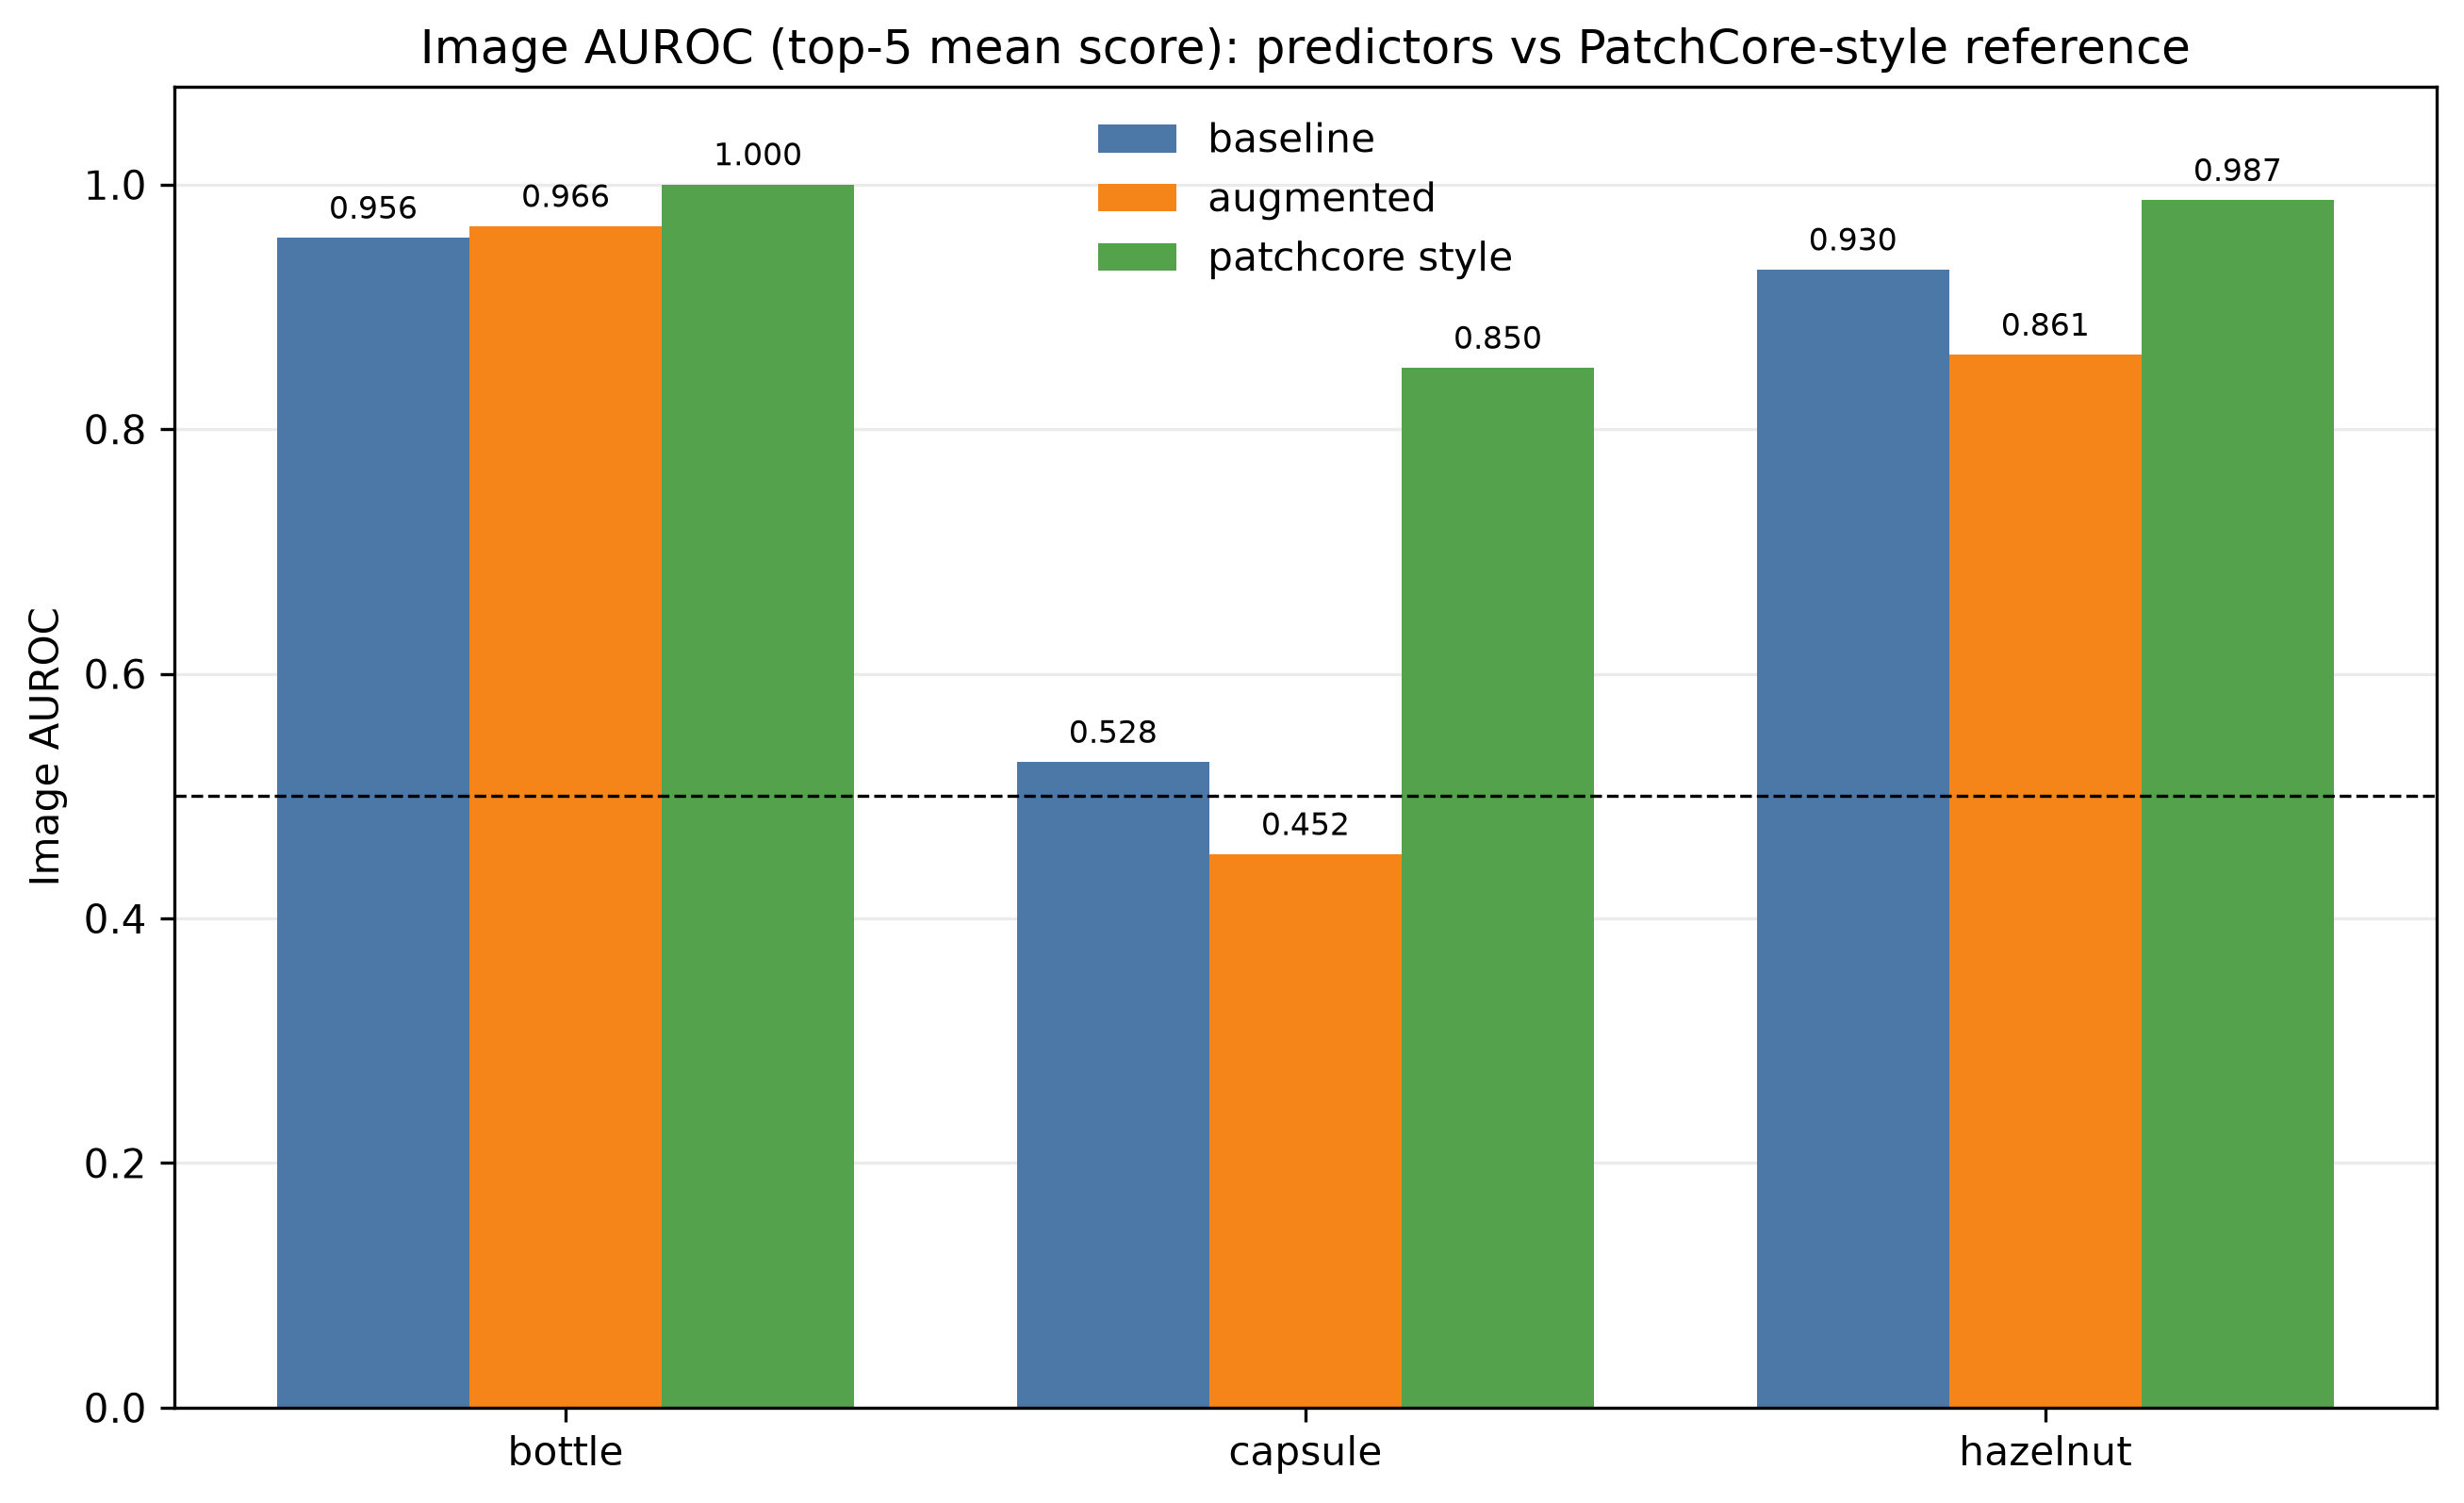
\includegraphics[width=0.85\textwidth]{figures/reference_comparison.png}
\caption{Image AUROC (top-5 mean score) of the baseline and augmented
predictors versus the nearest-neighbour reference on the test split.}
\label{fig:ref}
\end{figure}

\subsection{Masking policy: accuracy versus cost}

Table~\ref{tab:modes} compares the masking policies with the same baseline
predictors. Fixed, default-adaptive and dense masking give nearly identical
localisation (mean pixel AUROC 0.840, 0.840 and 0.848) while dense masking
needs $196/16=12.25\times$ as many predictor passes. Default-adaptive uses
only 16.1 masks per image, a 91.8\,\% reduction from dense. This saving is
almost entirely because the default gate opens on only about one test image
in a hundred (1.2\,\%, 0\,\% and 0.9\,\% for bottle, capsule, hazelnut), so
the method behaves like fixed coarse masking.

\begin{table}[H]
\centering
\caption{Pixel AUROC and AUPRO per category (B/C/H = bottle/capsule/hazelnut)
and mean predictor passes per image for four masking policies (baseline
predictors, test split).}
\label{tab:modes}
\resizebox{\textwidth}{!}{%
\begin{tabular}{lccccccc}
\hline
 & \multicolumn{3}{c}{\textbf{Pixel AUROC}} & \multicolumn{3}{c}{\textbf{AUPRO}} & \textbf{Masks} \\
\textbf{Policy} & B & C & H & B & C & H & \textbf{(mean)} \\
\hline
Fixed (coarse only)  & .930 & .685 & .907 & .766 & .098 & .578 & 16.0 \\
Adaptive, $\tau{=}0.5$ & .930 & .685 & .907 & .766 & .098 & .577 & 16.1 \\
Adaptive, cal.\ $\tau$ & .926 & .700 & .923 & .732 & .103 & .566 & 34.7 \\
Dense (196 masks)    & .928 & .706 & .909 & .762 & .111 & .584 & 196 \\
\hline
\end{tabular}%
}

\end{table}

\begin{figure}[H]
\centering
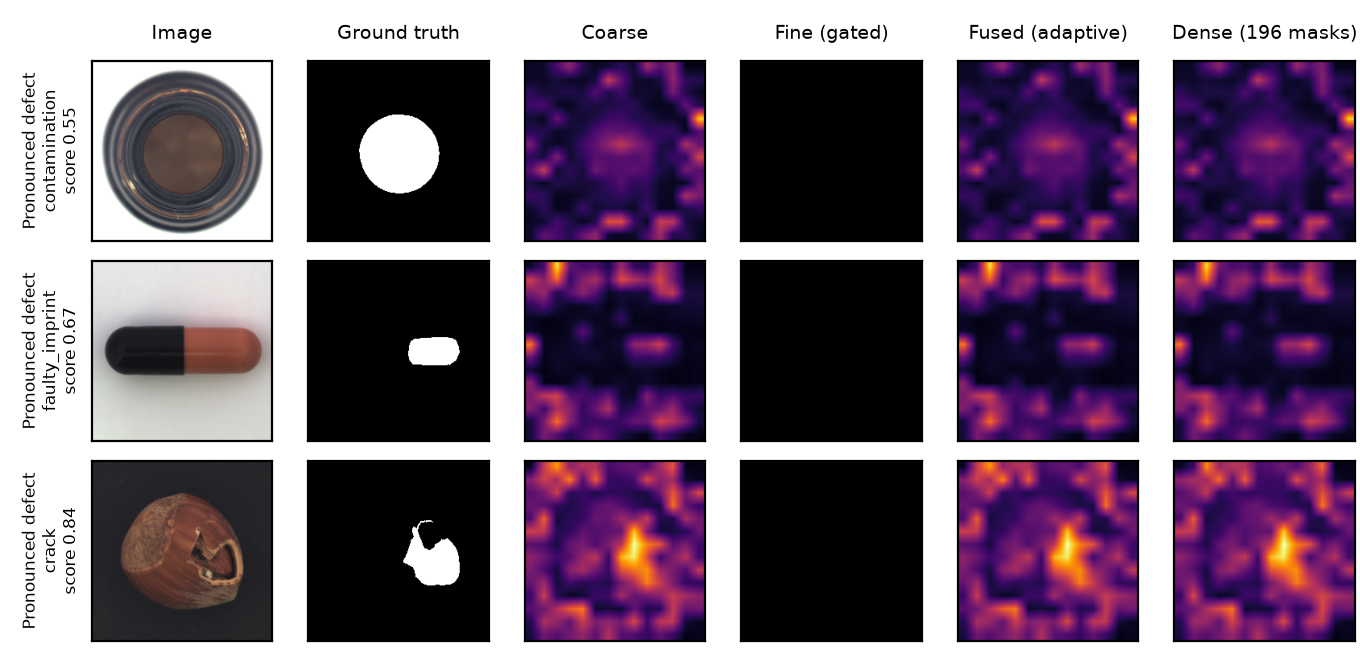
\includegraphics[width=0.98\textwidth]{figures/heatmaps_composite.png}
\caption{Raw cosine-discrepancy maps for one pronounced defect per category
(top to bottom: bottle, capsule, hazelnut). Columns: image, ground truth,
coarse map, gated fine map, fused adaptive map and the dense reference.}
\label{fig:heat}
\end{figure}

Figure~\ref{fig:heat} shows qualitative maps. For hazelnut the crack is
clearly highlighted by both the coarse and the dense maps. For the bottle
contamination the discrepancy is spread diffusely and is weaker than the
response at the image border, which hurts image-level ranking. For capsule
the faulty imprint is only weakly highlighted, consistent with chance-level
image AUROC.

\subsection{Latency and memory}

Table~\ref{tab:latency} gives the cost on the 8~GB RTX 4060. The frozen
encoder dominates: 3.94~GB of weights and 87.5~ms per image, with a peak
memory of 4.08~GB, so the pipeline fits an 8~GB card. Adaptive masking adds
8.9~ms over fixed masking end to end (133.8 against 124.9~ms), while dense
masking is $2.6\times$ slower than adaptive (349.8~ms).

\begin{table}[H]
\centering
\caption{Latency and memory on an RTX 4060 (8~GB), FP32 encoder. End-to-end
time is the mean $\pm$ standard deviation over 40 images; the last column is
predictor-only scoring on cached latents per category (bottle/capsule/hazelnut).}
\label{tab:latency}
\resizebox{\textwidth}{!}{%
\begin{tabular}{lccc}
\hline
\textbf{Policy} & \textbf{End-to-end (ms)} & \textbf{P95 (ms)} & \textbf{Scoring only B/C/H (ms)} \\
\hline
Encoder only (batch 1) & $87.5\pm5.4$  & 100.5 & -- \\
Fixed    & $124.9\pm3.5$  & 130.2 & 18.1 / 17.5 / 17.5 \\
Adaptive & $133.8\pm4.4$  & 141.3 & 30.4 / 20.6 / 21.1 \\
Dense    & $349.8\pm10.1$ & 367.9 & 214.4 / 216.7 / 238.1 \\
\hline
\multicolumn{4}{l}{Peak GPU memory: 4078~MB (all three policies); encoder weights 3939~MB.}
\end{tabular}%
}

\end{table}

\begin{figure}[H]
\centering
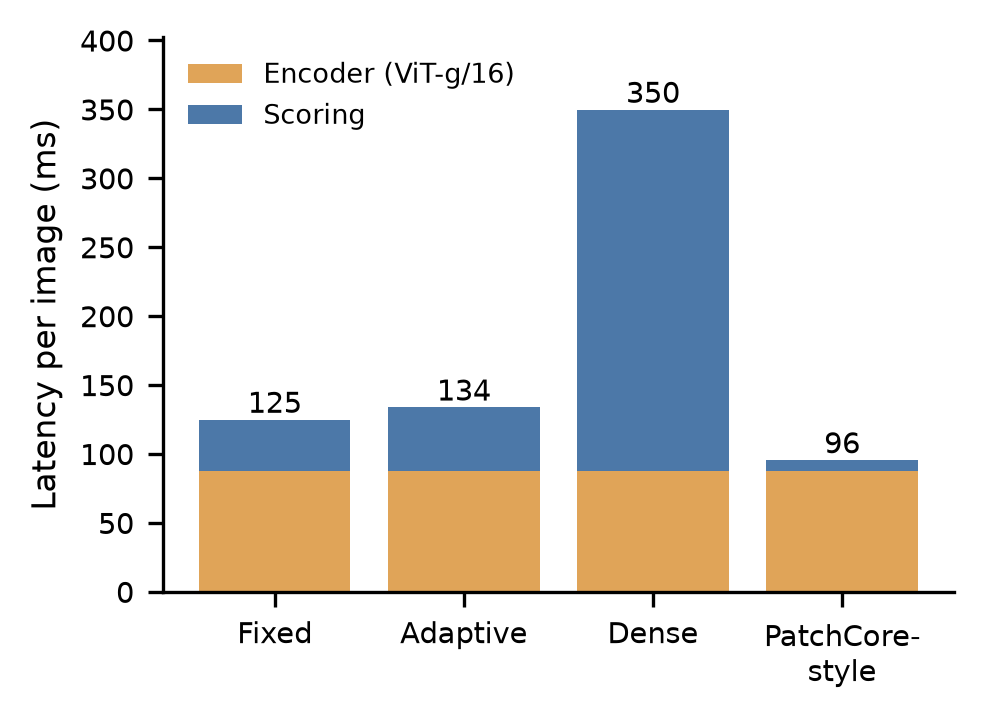
\includegraphics[width=0.75\textwidth]{figures/latency_e2e.png}
\caption{End-to-end latency per image split into encoder and scoring time.}
\label{fig:lat}
\end{figure}

\subsection{Validation-only gate calibration}

The default gate is inactive and the max-patch image score lets a single
noisy patch decide an image. Calibrating the gate threshold from the
$q$-quantile of nominal validation region scores (Table~\ref{tab:gate}) and
using a top-5 mean image score were declared before any test result was
inspected. The calibrated setting lifts the mean image AUROC from 0.750 to
0.796 and the mean pixel AUROC from 0.840 to 0.850, at 34.7 masks per image
instead of 16.1. Table~\ref{tab:bootorig} shows that the only statistically
supported improvement is the top-5 score on hazelnut; everywhere else the
interval contains zero.

\begin{table}[H]
\centering
\caption{Gate calibration on nominal validation images. For each category:
$\tau$ / fine windows per nominal image / \% of nominal images triggering a
fine pass.}
\label{tab:gate}
\resizebox{\textwidth}{!}{%
\begin{tabular}{lccc}
\hline
\textbf{Gate} & \textbf{Bottle} & \textbf{Capsule} & \textbf{Hazelnut} \\
\hline
Default        & .500 / 0.0 / 0   & .500 / 0.0 / 0    & .500 / 0.0 / 0 \\
$q=0.9$        & .098 / 19.8 / 86 & .207 / 19.6 / 91 & .279 / 19.7 / 92 \\
$q=0.95$       & .123 / 9.9 / 62  & .225 / 9.8 / 68  & .307 / 9.8 / 74 \\
$q=0.99$       & .158 / 2.3 / 19  & .264 / 2.2 / 23  & .350 / 2.1 / 23 \\
$q=0.995$      & .184 / 1.1 / 14  & .282 / 1.1 / 14  & .368 / 1.0 / 13 \\
\hline
\end{tabular}%
}

\end{table}

\begin{table}[H]
\centering
\caption{Paired-bootstrap change in image AUROC versus the original pipeline
(default gate, max score), 95\,\% interval. Asterisk: interval excludes zero.}
\label{tab:bootorig}
\resizebox{\textwidth}{!}{%
\begin{tabular}{lccc}
\hline
\textbf{Category} & \textbf{Gate only} & \textbf{Top-5 only} & \textbf{Both (primary)} \\
\hline
Bottle   & +.026 [$-$.037, +.097] & +.032 [$-$.005, +.078] & +.030 [$-$.026, +.097] \\
Capsule  & +.001 [$-$.114, +.107] & +.006 [$-$.126, +.153] & +.022 [$-$.128, +.180] \\
Hazelnut & +.009 [$-$.055, +.069] & +.128 [+.068, +.198]\textsuperscript{*} & +.088 [+.006, +.171]\textsuperscript{*} \\
\hline
\end{tabular}%
}

\end{table}

\section{Results of the Validation-Selected Improvements}

\subsection{Selecting on synthetic defects}

Figure~\ref{fig:synth} shows examples of the synthetic defects. For the
final-layer predictor the selection protocol chose a per-token-position
z-score of the patch score (each of the 196 positions normalised with the
mean and standard deviation of nominal validation scores), $\sigma=0$, $k=3$,
$\lambda=1$ and the default gate. After the selection was saved, the
proxy's ranking of eight scoring variants agreed with the test split (mean
Spearman correlation 0.74 for image AUROC with the max score, 0.86 with
top-5, 0.84 for pixel AUROC and 0.94 for AUPRO) but only weakly for
capsule's max-score image AUROC (0.42).

\begin{figure}[H]
\centering
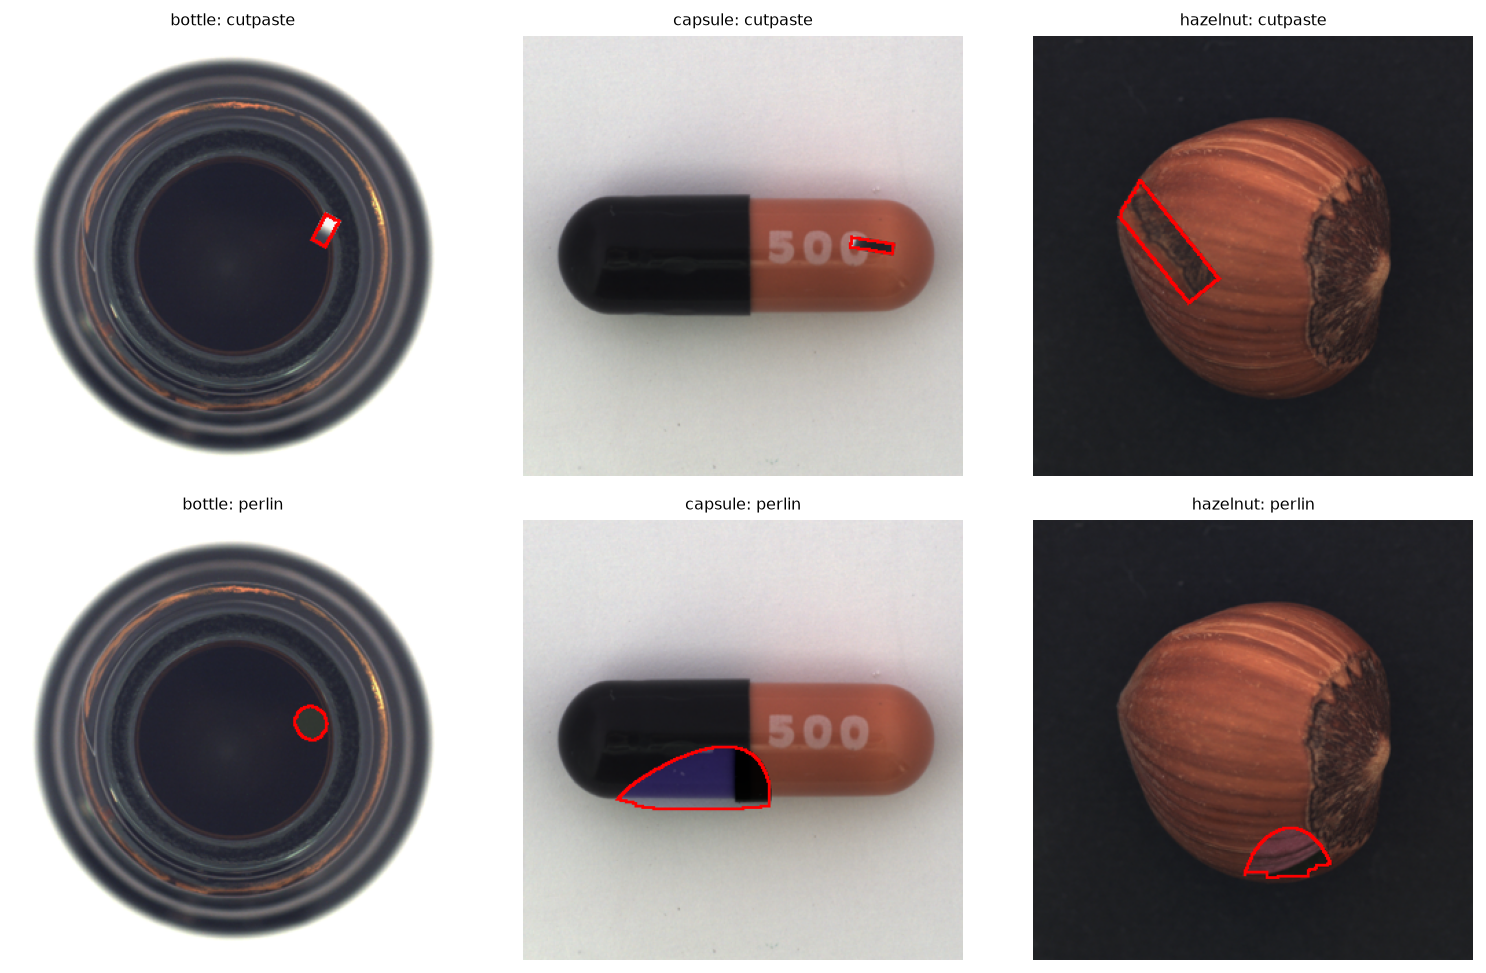
\includegraphics[width=0.85\textwidth]{figures/synthetic_examples.png}
\caption{Synthetic validation defects (CutPaste and Perlin-noise blends) on
nominal validation images; the defect outline is shown in red.}
\label{fig:synth}
\end{figure}

For the encoder layer, mid layers were best on the synthetic criterion (0.987
for layers 24 and 28, 0.986 for layer 32 and 0.969 for the final cached
latents). The declared rule selected layer 32; layers 24 and 28 are within
the tie margin.

\subsection{Effect on the test split}

Table~\ref{tab:improved} and Table~\ref{tab:bootimp} report the official
test split, with one scoring pass per row. Position z-scoring alone (final
layer) raises mean pixel AUROC from 0.840 to 0.941 and mean AUPRO from 0.480
to 0.717. Moving the predictor to layer 32 on top of it raises capsule top-3
image AUROC from 0.672 to 0.767 (+0.095, interval [+0.038, +0.150]) and
hazelnut from 0.939 to 0.993 (+0.054, [+0.017, +0.101]); bottle is at the
ceiling. The combination improves image AUROC over the original pipeline in
all three categories (bottle +0.075, capsule +0.246, hazelnut +0.191; all
intervals exclude zero) with the same 16.0--16.6 masks per image and a
scorer latency of about 22~ms per image. Mean pixel AUROC reaches 0.962 and
mean AUPRO 0.813.

\begin{table}[H]
\centering
\caption{Test results after the validation-selected changes. Img AUROC is
given for the max score and for the mean of the top-3 token scores.
(a)~Layer-32 settings re-selected on synthetic data (Mahalanobis residual
score, max score); (b)~nearest-neighbour reference on layer-32 tokens (full
memory bank), context only.}
\label{tab:improved}
\resizebox{\textwidth}{!}{%
\begin{tabular}{llccccc}
\hline
\textbf{Category} & \textbf{Method} & \textbf{Img AUROC (max)} & \textbf{Img AUROC (top-3)} & \textbf{Pixel AUROC} & \textbf{AUPRO} & \textbf{Masks/img} \\
\hline
\multirow{6}{*}{Bottle}
 & Original baseline (final layer, $1-\cos$) & 0.925 & 0.952 & 0.930 & 0.766 & 16.2 \\
 & + position z-score (final layer) & 0.993 & 0.998 & 0.952 & 0.831 & 16.2 \\
 & Layer 32, $1-\cos$ & 0.959 & 0.975 & 0.979 & 0.904 & 16.2 \\
 & \textbf{Layer 32 + position z-score} & 0.994 & 0.999 & 0.966 & 0.871 & 16.2 \\
 & Layer 32 + Mahalanobis $d{=}128$\textsuperscript{a} & 0.991 & 0.998 & 0.983 & 0.928 & 16.2 \\
 & kNN reference, layer 32\textsuperscript{b} & 1.000 & 1.000 & 0.987 & 0.937 & -- \\
\hline
\multirow{6}{*}{Capsule}
 & Original baseline (final layer, $1-\cos$) & 0.522 & 0.512 & 0.684 & 0.098 & 16.0 \\
 & + position z-score (final layer) & 0.622 & 0.672 & 0.901 & 0.508 & 16.0 \\
 & Layer 32, $1-\cos$ & 0.543 & 0.660 & 0.836 & 0.309 & 16.0 \\
 & \textbf{Layer 32 + position z-score} & 0.721 & 0.767 & 0.931 & 0.666 & 16.0 \\
 & Layer 32 + Mahalanobis $d{=}128$\textsuperscript{a} & 0.600 & 0.647 & 0.956 & 0.720 & 16.0 \\
 & kNN reference, layer 32\textsuperscript{b} & 0.909 & 0.909 & 0.962 & 0.771 & -- \\
\hline
\multirow{6}{*}{Hazelnut}
 & Original baseline (final layer, $1-\cos$) & 0.802 & 0.897 & 0.907 & 0.577 & 16.1 \\
 & + position z-score (final layer) & 0.864 & 0.939 & 0.969 & 0.812 & 16.1 \\
 & Layer 32, $1-\cos$ & 0.946 & 0.989 & 0.986 & 0.877 & 16.6 \\
 & \textbf{Layer 32 + position z-score} & 0.981 & 0.993 & 0.989 & 0.901 & 16.6 \\
 & Layer 32 + Mahalanobis $d{=}128$\textsuperscript{a} & 0.960 & 0.969 & 0.987 & 0.894 & 16.6 \\
 & kNN reference, layer 32\textsuperscript{b} & 0.999 & 1.000 & 0.995 & 0.941 & -- \\
\hline
\multirow{6}{*}{Mean}
 & Original baseline (final layer, $1-\cos$) & 0.750 & 0.787 & 0.840 & 0.480 & 16.1 \\
 & + position z-score (final layer) & 0.826 & 0.870 & 0.941 & 0.717 & 16.1 \\
 & Layer 32, $1-\cos$ & 0.816 & 0.875 & 0.934 & 0.697 & 16.3 \\
 & \textbf{Layer 32 + position z-score} & 0.899 & 0.920 & 0.962 & 0.813 & 16.3 \\
 & Layer 32 + Mahalanobis $d{=}128$\textsuperscript{a} & 0.850 & 0.871 & 0.975 & 0.847 & 16.3 \\
 & kNN reference, layer 32\textsuperscript{b} & 0.969 & 0.970 & 0.981 & 0.883 & -- \\
\hline
\end{tabular}%
}

\end{table}

\begin{table}[H]
\centering
\caption{Paired-bootstrap change in image AUROC on the test split, 95\,\%
interval. Asterisk: interval excludes zero. The first four rows use
configurations fixed before their test evaluation; the last three evaluate
the layer-32 re-selection.}
\label{tab:bootimp}
\resizebox{\textwidth}{!}{%
\begin{tabular}{lccc}
\hline
\textbf{Comparison (new vs reference)} & \textbf{Bottle} & \textbf{Capsule} & \textbf{Hazelnut} \\
\hline
Final layer + z-score (top-3) vs original (max) & +0.073 [+0.019, +0.152]\textsuperscript{*} & +0.150 [$-$0.045, +0.356] & +0.137 [+0.054, +0.226]\textsuperscript{*} \\
Layer 32 + z-score (top-3) vs original (max) & +0.075 [+0.021, +0.153]\textsuperscript{*} & +0.246 [+0.049, +0.457]\textsuperscript{*} & +0.191 [+0.107, +0.284]\textsuperscript{*} \\
Layer 32 + z-score vs final layer + z-score (top-3) & +0.002 [+0.000, +0.007] & +0.095 [+0.038, +0.150]\textsuperscript{*} & +0.054 [+0.017, +0.101]\textsuperscript{*} \\
Layer 32, $1-\cos$ vs original (max) & +0.034 [$-$0.024, +0.110] & +0.021 [$-$0.075, +0.114] & +0.144 [+0.061, +0.239]\textsuperscript{*} \\
Layer 32 Mahalanobis vs layer 32 $1-\cos$ (max) & +0.033 [+0.004, +0.078]\textsuperscript{*} & +0.057 [$-$0.123, +0.259] & +0.013 [$-$0.031, +0.068] \\
Layer 32 Mahalanobis (max) vs layer 32 z-score (top-3) & $-$0.008 [$-$0.029, +0.002] & $-$0.167 [$-$0.282, $-$0.057]\textsuperscript{*} & $-$0.034 [$-$0.067, $-$0.007]\textsuperscript{*} \\
Layer 32 Mahalanobis (max) vs original (max) & +0.067 [+0.012, +0.144]\textsuperscript{*} & +0.079 [$-$0.134, +0.303] & +0.157 [+0.076, +0.254]\textsuperscript{*} \\
\hline
\end{tabular}%
}

\end{table}

\begin{figure}[H]
\centering
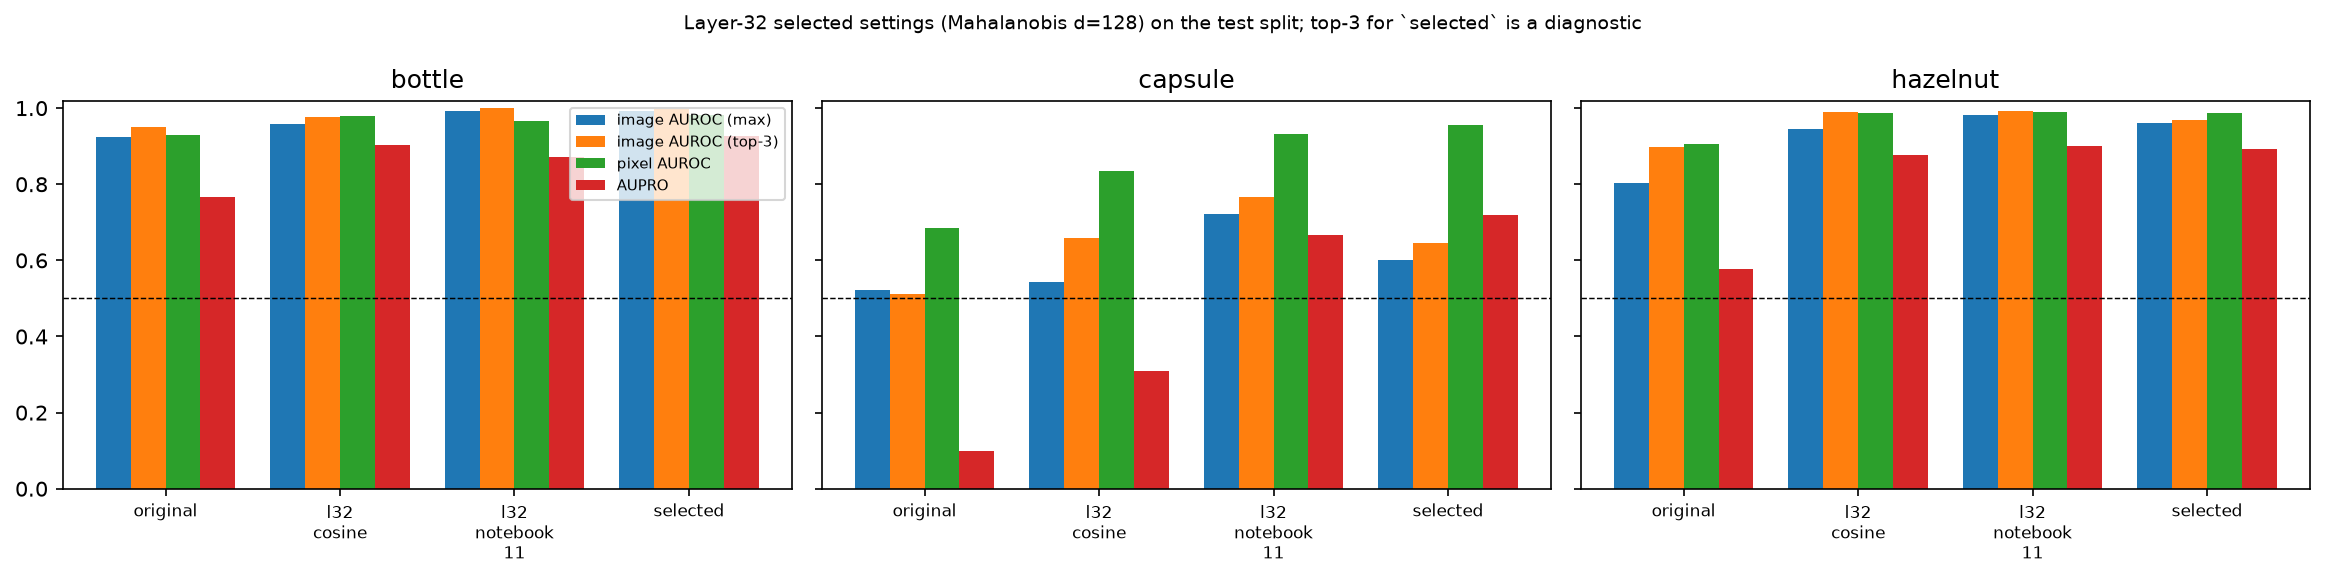
\includegraphics[width=0.98\textwidth]{figures/layer32_confirmation.png}
\caption{Layer-32 predictor with the selected Mahalanobis scoring on the test
split, compared with the other rows of Table~\ref{tab:improved}.}
\label{fig:l32}
\end{figure}

\subsection{A negative result: re-selection for layer 32}

Because the settings were chosen for the final-layer predictor, the same
protocol was repeated on the layer-32 predictors and synthetic data, again
without touching the test split. It chose a Mahalanobis residual score (PCA
to 128 components, fitted on nominal validation residuals) with the max
score, which was then scored once on the test split. Against raw cosine on
the same predictor it improves bottle (+0.033, [+0.004, +0.078]) and is
inconclusive for capsule and hazelnut, and its pixel AUROC and AUPRO are
higher (means 0.976 and 0.847, point estimates). At image level, however, it
is \emph{worse} than the z-score configuration (capsule $-0.167$,
[$-0.282$, $-0.057$]; hazelnut $-0.034$, [$-0.067$, $-0.007$]). The
configuration fixed before the re-selection is therefore reported as the
headline and the Mahalanobis result as a negative finding on how well
synthetic validation transfers.

\subsection{Pretrained predictor and context leakage}

Our masking acts on latents after full-image encoding, so context tokens may
already contain the defect. As a first test, Meta's pretrained I-JEPA
context encoder and predictor were run on the visible tokens only
(zero-shot, ImageNet-22K). It did not beat our predictor (image AUROC with
the z-score: bottle 0.986 against 0.998, capsule 0.647 against 0.672,
hazelnut 0.809 against 0.939) and costs about 980~ms per image against
23~ms. Leakage is therefore not supported as the main limit, but the test is
confounded by predictor size and training data.

\section{Discussion}

The pipeline is decoder-free, fits in 8~GB and runs end to end in 134~ms.
Latent prediction gives a usable localisation signal for categories with
regular structure, and the coarse scheme obtains nearly the same
localisation as dense masking with 8\,\% of the predictor passes. The
adaptive fine pass did not add accuracy with the default gate and added only
inconsistent gains with a calibrated gate, so its value in this pilot is
limited to avoiding dense masking, which fixed masking also achieves.

The largest gains came not from the masking policy but from the input
features and the score normalisation: mid-level tokens (layer 32) and a
per-position z-score recover much of the gap to the nearest-neighbour
reference and lift capsule from chance level to 0.77 image AUROC. A
nearest-neighbour reference on the same layer-32 tokens remains stronger at
image level (mean 0.97 against 0.92), so the gap to a memory-bank method is
reduced, not closed. The re-selection experiment shows that a synthetic
validation criterion close to its ceiling can prefer settings that do not
transfer to image-level test performance.

\section{Limitations}

\begin{itemize}[leftmargin=*]
    \item \textbf{Scope.} Only 3 of 15 categories were evaluated; the other
    12, MVTec AD 2 and a faithful PatchCore and MAE baseline are outstanding.
    \item \textbf{Sample size and seeds.} Validation sets have 21--39 images
    and test sets 20--40 normal images, and each predictor is a single
    training run per category, so differences of a few points are within
    noise.
    \item \textbf{Synthetic validation.} CutPaste and Perlin defects are a
    stand-in for real defects; no proxy-versus-test check exists for layer
    32.
    \item \textbf{Possible context leakage.} Masking after full-image
    encoding was only tested zero-shot; retraining on input-masked latents
    was not done.
    \item \textbf{Reference baseline.} The nearest-neighbour row is not the
    original PatchCore.
    \item \textbf{Latency scope.} Cached-latent scoring excludes encoding and
    single-run latencies vary between sessions.
    \item \textbf{Validation reuse.} The same validation images are used for
    early stopping, calibration and selection, which makes false-positive
    control slightly optimistic.
\end{itemize}

% ------------------------------------------------------------
% CHAPTER 6
% ------------------------------------------------------------
\chapterseparator
\chapter{Conclusion and Future Scope}

\section{Conclusion}

This project built and evaluated I-JEPA-AD, a decoder-free anomaly detector
that predicts masked regions in the latent space of a frozen I-JEPA ViT-g/16
and refines suspicious regions with a gated fine pass. On a three-category
MVTec AD pilot it localises defects with a mean pixel AUROC of 0.84 using 16
predictor passes per image and 134~ms end-to-end latency on an 8~GB GPU, a
$2.6\times$ speed-up over dense masking at equal localisation quality. The
adaptive gate did not give a consistent accuracy benefit, capsule defects
were not detected by the original pipeline, and a nearest-neighbour baseline
on the same latents was stronger.

Choosing the encoder layer and the score normalisation on synthetic defects,
without the test split, then gave large gains: with the same 16 masks per
image the mean pixel AUROC rose to 0.96, the mean AUPRO from 0.48 to 0.81
and the mean top-3 image AUROC to 0.92, with paired-bootstrap improvements
over the original pipeline in every category and capsule rising from near
chance to 0.77. A nearest-neighbour reference on the same tokens remains
stronger at image level, and a layer-32 re-selection did not transfer to the
test split at image level. Validation-only selection with bootstrap
intervals makes these conclusions auditable.

\section{Future Scope}

\begin{itemize}[leftmargin=*]
    \item Evaluate the remaining twelve MVTec AD categories and MVTec AD 2
    with multiple seeds and a validation-locked configuration.
    \item Train predictors on layers 24 and 28 and on layer concatenations,
    and study mask block size, augmentation and training length on the
    synthetic validation set.
    \item Retrain on input-masked context latents to measure context leakage
    decisively.
    \item Add a faithful PatchCore and MAE baseline under the same protocol.
    \item Investigate higher input resolution or an object crop for capsule,
    which changes the token grid and needs more memory and engineering.
\end{itemize}

% ============================================================
% REFERENCES
% ============================================================
\clearpage
\addcontentsline{toc}{chapter}{References}
\begin{thebibliography}{99}

\bibitem{assran2023ijepa} M. Assran, Q. Duval, I. Misra, P. Bojanowski, P. Vincent, M. Rabbat, Y. LeCun, and N. Ballas, ``Self-supervised learning from images with a joint-embedding predictive architecture,'' in \textit{Proc. IEEE/CVF Conf. Comput. Vis. Pattern Recognit. (CVPR)}, 2023, pp. 15619--15629.

\bibitem{he2022mae} K. He, X. Chen, S. Xie, Y. Li, P. Doll\'ar, and R. Girshick, ``Masked autoencoders are scalable vision learners,'' in \textit{Proc. IEEE/CVF Conf. Comput. Vis. Pattern Recognit. (CVPR)}, 2022, pp. 16000--16009.

\bibitem{bergmann2019mvtec} P. Bergmann, M. Fauser, D. Sattlegger, and C. Steger, ``MVTec AD --- a comprehensive real-world dataset for unsupervised anomaly detection,'' in \textit{Proc. IEEE/CVF Conf. Comput. Vis. Pattern Recognit. (CVPR)}, 2019, pp. 9592--9600.

\bibitem{bergmann2021mvtec} P. Bergmann, K. Batzner, M. Fauser, D. Sattlegger, and C. Steger, ``The MVTec anomaly detection dataset: A comprehensive real-world dataset for unsupervised anomaly detection,'' \textit{Int. J. Comput. Vis.}, vol. 129, no. 4, pp. 1038--1059, 2021.

\bibitem{roth2022patchcore} K. Roth, L. Pemula, J. Zepeda, B. Sch\"olkopf, T. Brox, and P. Gehler, ``Towards total recall in industrial anomaly detection,'' in \textit{Proc. IEEE/CVF Conf. Comput. Vis. Pattern Recognit. (CVPR)}, 2022, pp. 14318--14328.

\bibitem{defard2021padim} T. Defard, A. Setkov, A. Loesch, and R. Audigier, ``PaDiM: A patch distribution modeling framework for anomaly detection and localization,'' in \textit{Int. Conf. Pattern Recognit. (ICPR) Workshops}, 2021, pp. 475--489.

\bibitem{zavrtanik2021draem} V. Zavrtanik, M. Kristan, and D. Sko\v{c}aj, ``DRAEM --- a discriminatively trained reconstruction embedding for surface anomaly detection,'' in \textit{Proc. IEEE/CVF Int. Conf. Comput. Vis. (ICCV)}, 2021, pp. 8330--8339.

\bibitem{zavrtanik2021inpainting} V. Zavrtanik, M. Kristan, and D. Sko\v{c}aj, ``Reconstruction by inpainting for visual anomaly detection,'' \textit{Pattern Recognit.}, vol. 112, art. 107706, 2021.

\bibitem{li2021cutpaste} C.-L. Li, K. Sohn, J. Yoon, and T. Pfister, ``CutPaste: Self-supervised learning for anomaly detection and localization,'' in \textit{Proc. IEEE/CVF Conf. Comput. Vis. Pattern Recognit. (CVPR)}, 2021, pp. 9664--9674.

\bibitem{batzner2024efficientad} K. Batzner, L. Heckler, and R. K\"onig, ``EfficientAD: Accurate visual anomaly detection at millisecond-level latencies,'' in \textit{Proc. IEEE/CVF Winter Conf. Appl. Comput. Vis. (WACV)}, 2024, pp. 128--138.

\bibitem{akcay2022anomalib} S. Akcay, D. Ameln, A. Vaidya, B. Lakshmanan, N. Ahuja, and U. Genc, ``Anomalib: A deep learning library for anomaly detection,'' in \textit{Proc. IEEE Int. Conf. Image Process. (ICIP)}, 2022, pp. 1706--1710.

\bibitem{lecun2022path} Y. LeCun, ``A path towards autonomous machine intelligence, version 0.9.2,'' OpenReview, 2022.

\end{thebibliography}

% ============================================================
% APPENDICES
% ============================================================
\appendix

\chapter{Publications and Intellectual Property}

This annexure records project-related publications and intellectual
property.

\begin{table}[H]
\centering
\caption{Publications and Intellectual Property}
\begin{tabular}{p{0.15\textwidth}p{0.42\textwidth}p{0.25\textwidth}}
\toprule
Type & Title / Description & Status\\
\midrule
Research Paper & I-JEPA-AD: Decoder-Free Latent Anomaly Detection with Coarse-to-Fine Adaptive Masking (IEEE conference format) & Manuscript prepared; submission status to be updated\\
\bottomrule
\end{tabular}
\end{table}

\chapter{Student Contribution Statement}

Each student should provide a specific and verifiable description of their
contribution. The entries below are to be completed by the students.

\begin{longtable}{p{0.25\textwidth}p{0.20\textwidth}p{0.45\textwidth}}
\caption{Student Contribution Statement}\\
\toprule
Student Name & Roll Number & Contribution\\
\midrule
\endfirsthead
\toprule
Student Name & Roll Number & Contribution\\
\midrule
\endhead
Aryan Jawanjal & A-35 & \\
Akshat Tiwari & A-11 & \\
Arnav Milmile & A-30 & \\
Aashutosh Dubey & A-02 & \\
\bottomrule
\end{longtable}

\chapter{Project Outputs}

Major outputs of the project:

\begin{itemize}
    \item Software: the \texttt{ijepa\_ad} package, training and evaluation
    scripts, the Streamlit dashboard and 376 automated tests.
    \item Trained predictors for bottle, capsule and hazelnut for both the
    final-layer and the layer-32 tokens.
    \item Notebooks 05 to 13 documenting every experiment, with saved result
    files, the synthetic validation set generator and the selection records.
    \item Project repository: \texttt{https://github.com/Auxilus08/I-JEPA-AD}.
    \item Research paper in IEEE conference format describing the method and
    results.
\end{itemize}

% ------------------------------------------------------------
% End document
% ------------------------------------------------------------
\end{document}
